% 1957 年全国卷第 5 题：三平行平面与公垂线中点。
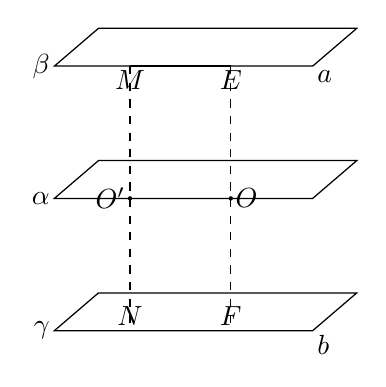
\begin{tikzpicture}[scale=0.8, line width=0.45pt,
  every node/.style={inner sep=1.5pt}]
  \coordinate (A1) at (-2,2.4); \coordinate (B1) at (2.1,2.4);
  \coordinate (C1) at (2.8,3.0); \coordinate (D1) at (-1.3,3.0);
  \coordinate (A2) at (-2,0.3); \coordinate (B2) at (2.1,0.3);
  \coordinate (C2) at (2.8,0.9); \coordinate (D2) at (-1.3,0.9);
  \coordinate (A3) at (-2,-1.8); \coordinate (B3) at (2.1,-1.8);
  \coordinate (C3) at (2.8,-1.2); \coordinate (D3) at (-1.3,-1.2);
  \coordinate (M) at (-0.8,2.4); \coordinate (E) at (0.8,2.4);
  \coordinate (Oprime) at (-0.8,0.3); \coordinate (O) at (0.8,0.3);
  \coordinate (N) at (-0.8,-1.8); \coordinate (F) at (0.8,-1.8);
  \draw (A1)--(B1)--(C1)--(D1)--cycle;
  \draw (A2)--(B2)--(C2)--(D2)--cycle;
  \draw (A3)--(B3)--(C3)--(D3)--cycle;
  \draw[dashed] (M)--(Oprime)--(N) (E)--(O)--(F);
  \draw (M)--(E) (N)--(F);
  \fill (Oprime) circle (0.035) (O) circle (0.035);
  \node[anchor=east] at (A1) {$\beta$};
  \node[anchor=east] at (A2) {$\alpha$};
  \node[anchor=east] at (A3) {$\gamma$};
  \node[anchor=north] at (M) {$M$};
  \node[anchor=north] at (E) {$E$};
  \node[anchor=south] at (N) {$N$};
  \node[anchor=south] at (F) {$F$};
  \node[anchor=east] at (Oprime) {$O'$};
  \node[anchor=west] at (O) {$O$};
  \node[anchor=north west] at (B1) {$a$};
  \node[anchor=north west] at (B3) {$b$};
\end{tikzpicture}
